\documentclass[12pt,a4paper]{article}

\usepackage[utf8]{inputenc}
\usepackage{graphicx}
\usepackage{amsmath}
\usepackage{amssymb}
\usepackage[hidelinks]{hyperref}
\usepackage{geometry}
\usepackage{float}
\usepackage{caption}
\usepackage{subcaption}

\geometry{
    left=25mm,
    right=25mm,
    top=25mm,
    bottom=25mm
}

% Title Page Information
\title{\textbf{MMI712 Project Phase 1 Report}}
\author{Okan Berhoglu 2739050}
\date{\today}

\begin{document}

% Title Page
\maketitle
\thispagestyle{empty}
\newpage

\tableofcontents
\newpage

\begin{abstract}
    \textit{This report describes the implementation of a Visual Question Answering (VQA) system using the Moondream model. The application is containerized with Docker to ensure easy deployment and reproducibility. A command-line interface (CLI) allows users to ask questions about images. The project demonstrates how to run efficient vision-language models on local hardware.}
\end{abstract}

\section{Introduction}
Recent advancements in Artificial Intelligence have led to the development of powerful Vision Language Models (VLMs) capable of understanding and generating text based on visual inputs. Models such as GPT-4V and Gemini have demonstrated remarkable capabilities in tasks ranging from image captioning to complex visual reasoning. Despite their performance, these state-of-the-art models often present significant challenges for practical deployment. Many are proprietary, limiting accessibility and research transparency. Furthermore, their substantial computational requirements make them unsuitable for resource-constrained environments, such as edge devices or local applications where latency and privacy are critical concerns. This necessitates the exploration of efficient, open-source alternatives that balance performance with resource utilization.

Moondream emerges as a compelling solution in this landscape. It is a small, open-source vision language model designed to run efficiently on consumer-grade hardware and even mobile devices. By leveraging a compact architecture, Moondream significantly reduces the computational overhead associated with traditional VLMs without sacrificing essential capabilities. Consequently, Moondream offers a practical pathway for deploying visual understanding capabilities in real-world scenarios where resource efficiency and accessibility are paramount. 

To ensure reproducibility and streamline the deployment process, Docker is utilized to containerize the application. Docker provides a lightweight and portable environment that encapsulates the application and its dependencies, eliminating the "it works on my machine" problem. By defining the runtime environment in a Dockerfile, we ensure that the model behaves consistently across different computing platforms. This approach simplifies the setup process for other researchers and developers, allowing them to easily deploy and experiment with software applications or models without worrying about conflicting libraries or system configurations.

In this work, the Moondream model is implemented for Visual Question Answering (VQA) tasks. The model processes natural language questions about input images and generates corresponding natural language answers. To ensure consistency and ease of deployment, the application is containerized using Docker. The implementation is validated using a set of test images and questions. The application is a web application that developed by using Streamlit.

This report is structured as follows; after the introduction, the methodology section describes the technical details of the implementation, an example usage of the application is given in the results section and the usage of the application is given in the usage section. Lastly the conclusion section provides a summary of the work done.

\section{Methodology}
The application is transformed into a web-based Visual Question Answering (VQA) system using the Streamlit framework. This shift from a command-line interface to a web application significantly enhances user interaction and accessibility. The core of the system remains the Moondream model, but the surrounding architecture is redesigned to support stateful user sessions, image management, and a responsive user interface.

\subsection{Application Architecture}
The application follows a modular structure, separating the user interface, business logic, and model interaction. The entry point is the \texttt{main.py} script, which serves as the main entry point for the Streamlit application. It initializes the session state, manages the navigation between different pages, and ensures the Moondream model is loaded. It directs the user to either the Main Page or the Chat Page based on the application state.

The User Interface, located in the \texttt{ui/} directory, is built using Streamlit's component-based design. It consists of the \texttt{MainPage} and \texttt{ChatPage} components. The \texttt{MainPage} handles the initial user landing, providing functionality for users to upload new images to start a chat session and displaying a history of recent chat sessions. The \texttt{ChatPage} manages the active chat interface, displaying the uploaded image, rendering the chat history (questions and answers), and providing an input field for new queries to interact with the model effectively.

To maintain clean code and separation of concerns, service modules are implemented in the \texttt{services/} directory. The \texttt{ChatService} manages the storage and retrieval of chat history, creating new sessions, and generating chat names. The \texttt{ImageService} handles image file operations, including saving uploaded images and loading them for display or processing.

\subsection{Model Integration}
The \texttt{Model} class in \texttt{model/model.py} encapsulates the interaction with the Moondream model. It is responsible for conditionally loading the model on GPU or CPU based on hardware availability, processing the input image into embeddings that the model can understand, and taking a natural language question and the encoded image to generate a text response during inference.

A dedicated script, \texttt{model\_installer.py}, is used to download the specific revision of the Moondream model from the Hugging Face hub. This ensures that the correct model files are present before the application starts, which is particularly important for the Dockerized environment.

\subsection{Containerization}
The application is containerized using Docker to ensure a consistent execution environment. The \texttt{Dockerfile} is updated to support the web application. It uses \texttt{python:3.10-slim} as a base image for a lightweight footprint and installs system dependencies and Python packages listed in \texttt{requirements.txt}, which now includes \texttt{streamlit}.

A crucial step in the methodology is the execution of \texttt{model\_installer.py} during the Docker build phase. This bakes the large model weights into the Docker image, preventing the need to download them every time the container starts.

Finally, the container exposes port 8501, the default for Streamlit, and uses \texttt{streamlit run main.py} as the entry point command.

\section{Usage}
\label{sec:usage}
The resulting image is published in the docker hub. The application can be found in this link:
\url{https://hub.docker.com/r/okanberhoglu/chat_moon_vlm}

After downloading the image, the application can be run using the following command:
\begin{center}
{\fontsize{12pt}{12pt}\selectfont
\texttt{docker run -p 8501:8501 okanberhoglu/chat\_moon\_vlm:latest}
}
\end{center}

The given command runs the Docker image in a container and maps the host's port 8501 to the container's port 8501. This allows the user to access the web application by navigating to \url{http://localhost:8501} in their web browser. The Docker image "okanberhoglu/chat\_moon\_vlm:latest" encapsulates all required dependencies, the Streamlit server, and the inference environment. Once the container is running, the application interface will be available for uploading images and asking questions.

\section{Results}
An example usage of the application and the results are given in this section. Firstly the test input image is given in the figure \ref{fig:test}.

\begin{figure}[H]
    \centering
    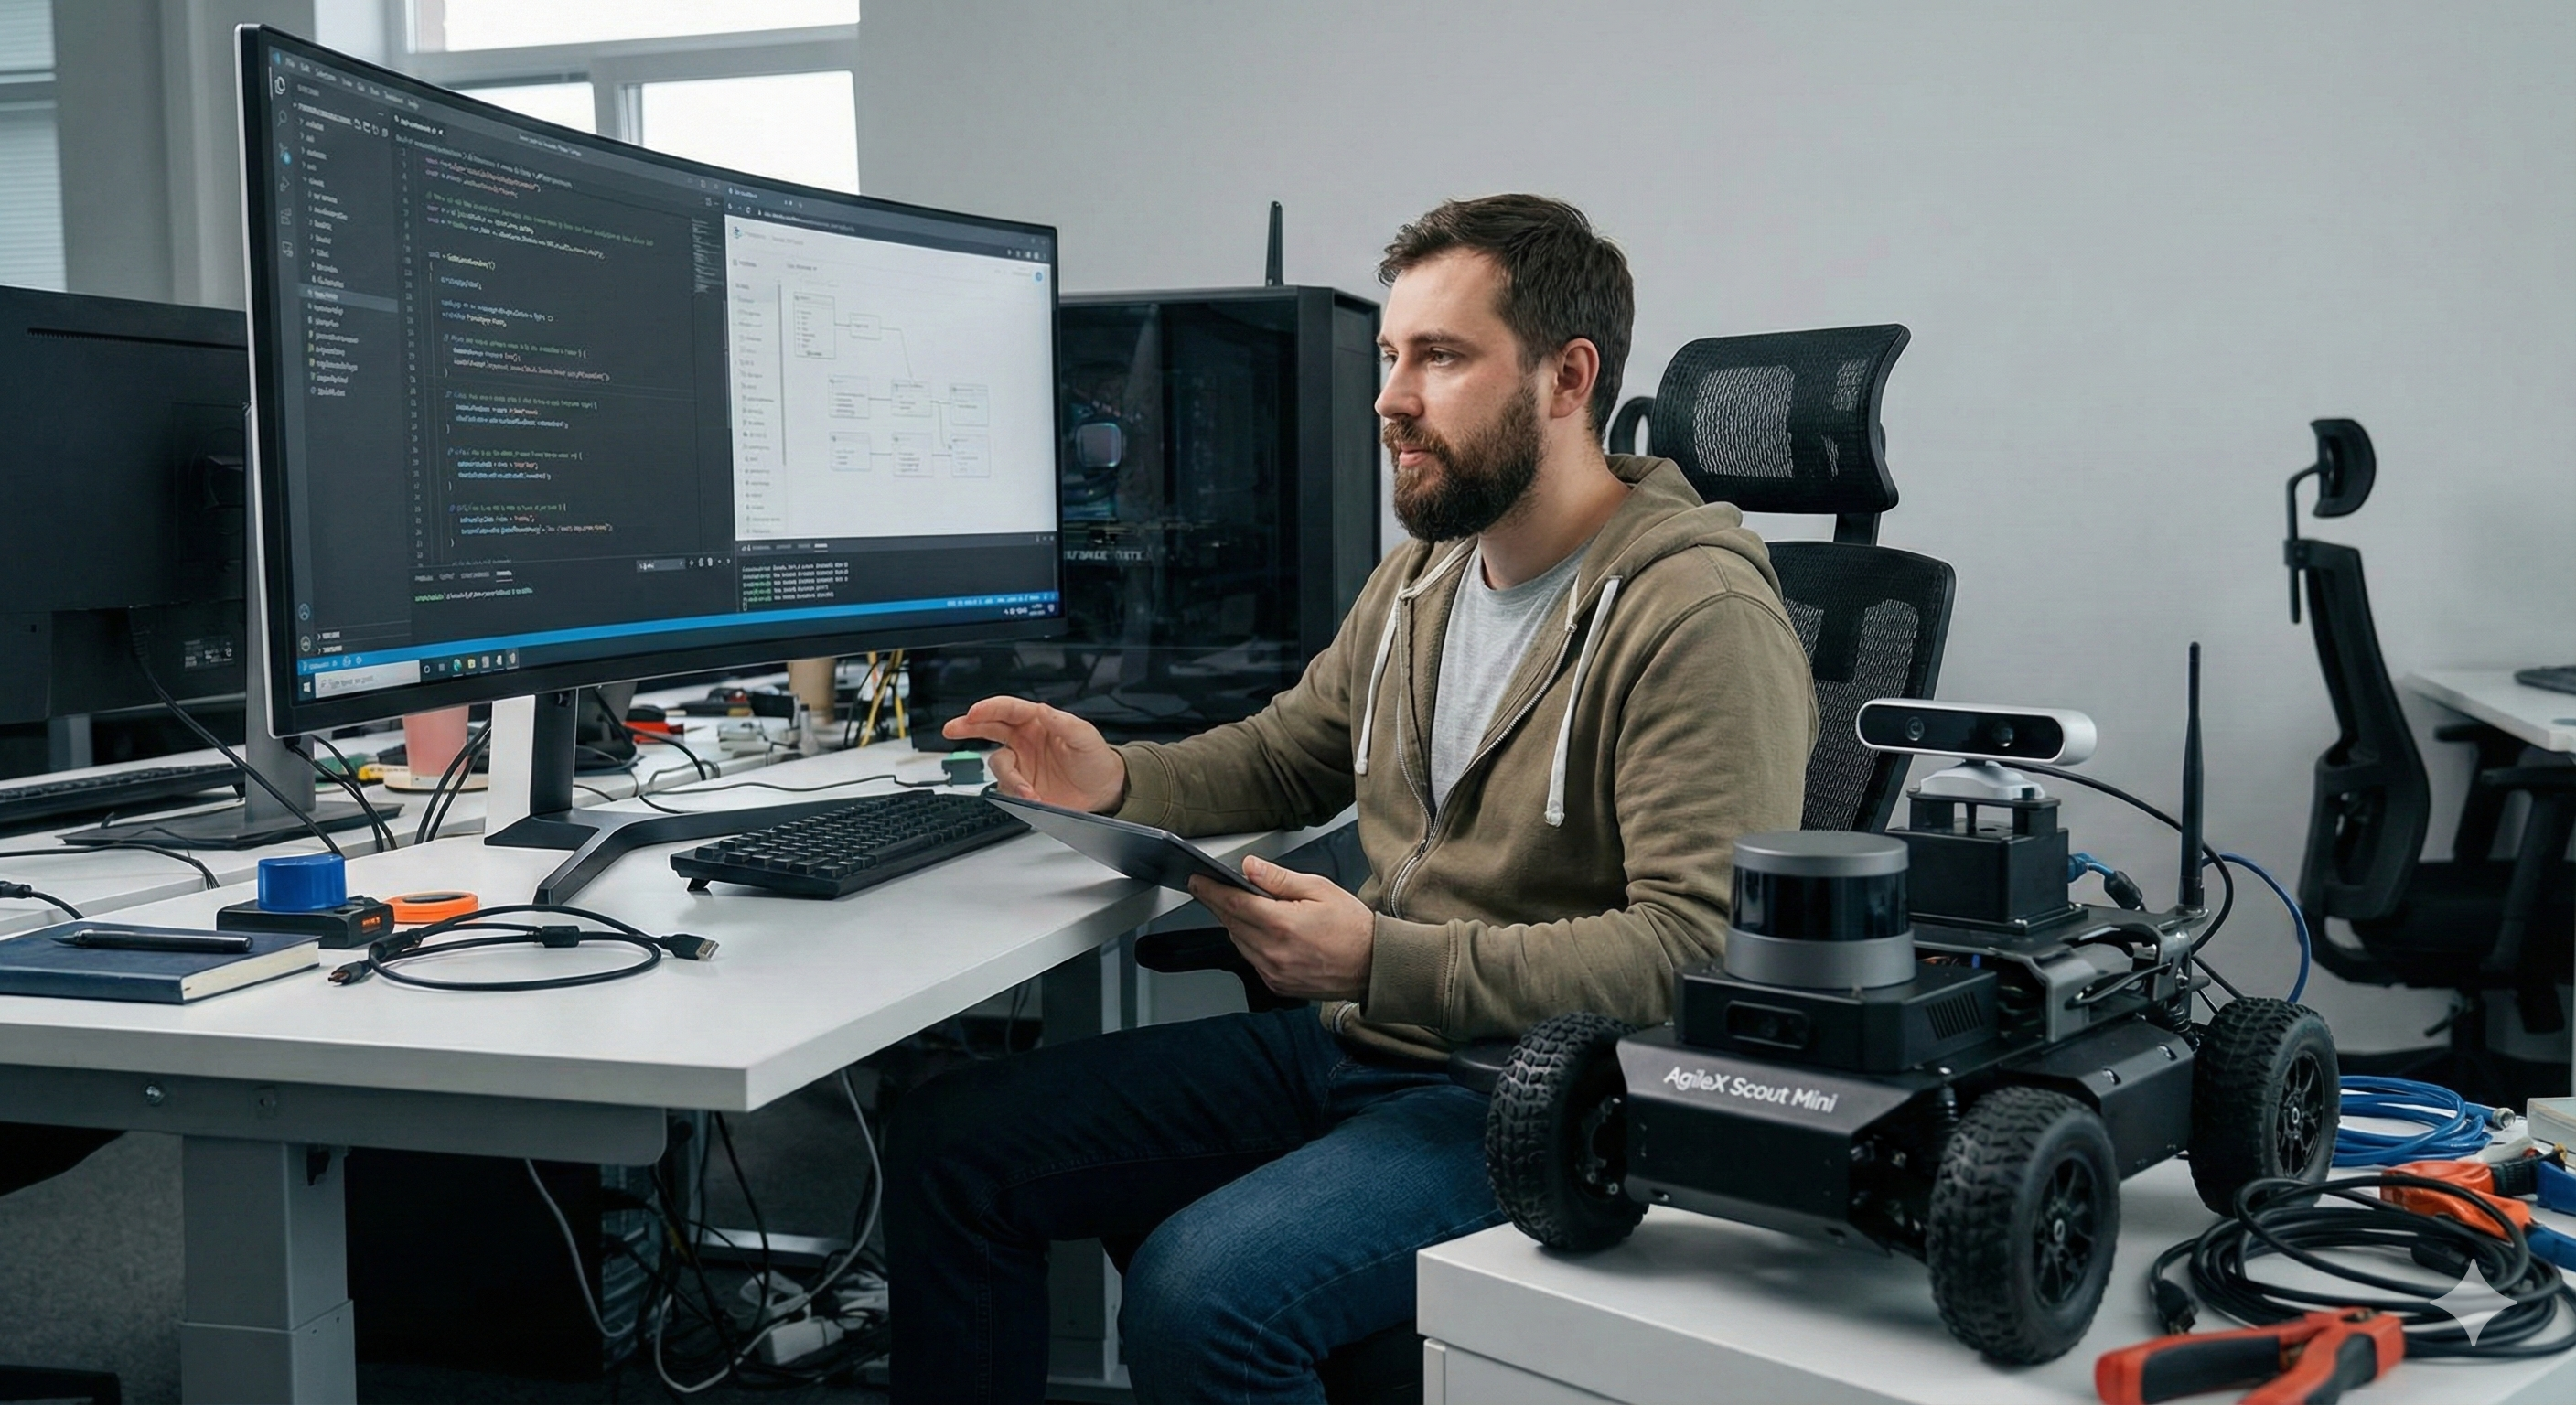
\includegraphics[width=350pt]{test_image.png}
    \caption{Example input image.}
    \label{fig:test}
\end{figure}
After running the application with the command given in the section \ref{sec:usage}, the application can be used as shown in the figures \ref{fig:q1} and \ref{fig:q2}.

\begin{figure}[H]
    \centering
    \includegraphics[width=400pt]{q1.png}
    \caption{Example usage.}
    \label{fig:q1}
\end{figure}
\begin{figure}[H]
    \centering
    \includegraphics[width=350pt]{q2.png}
    \caption{Example usage with questions.}
    \label{fig:q2}
\end{figure}

The application is executed with another test image which is given in the figure \ref{fig:test_two} as well. The results are given in the figure \ref{fig:two_q1}.

\begin{figure}[H]
    \centering
    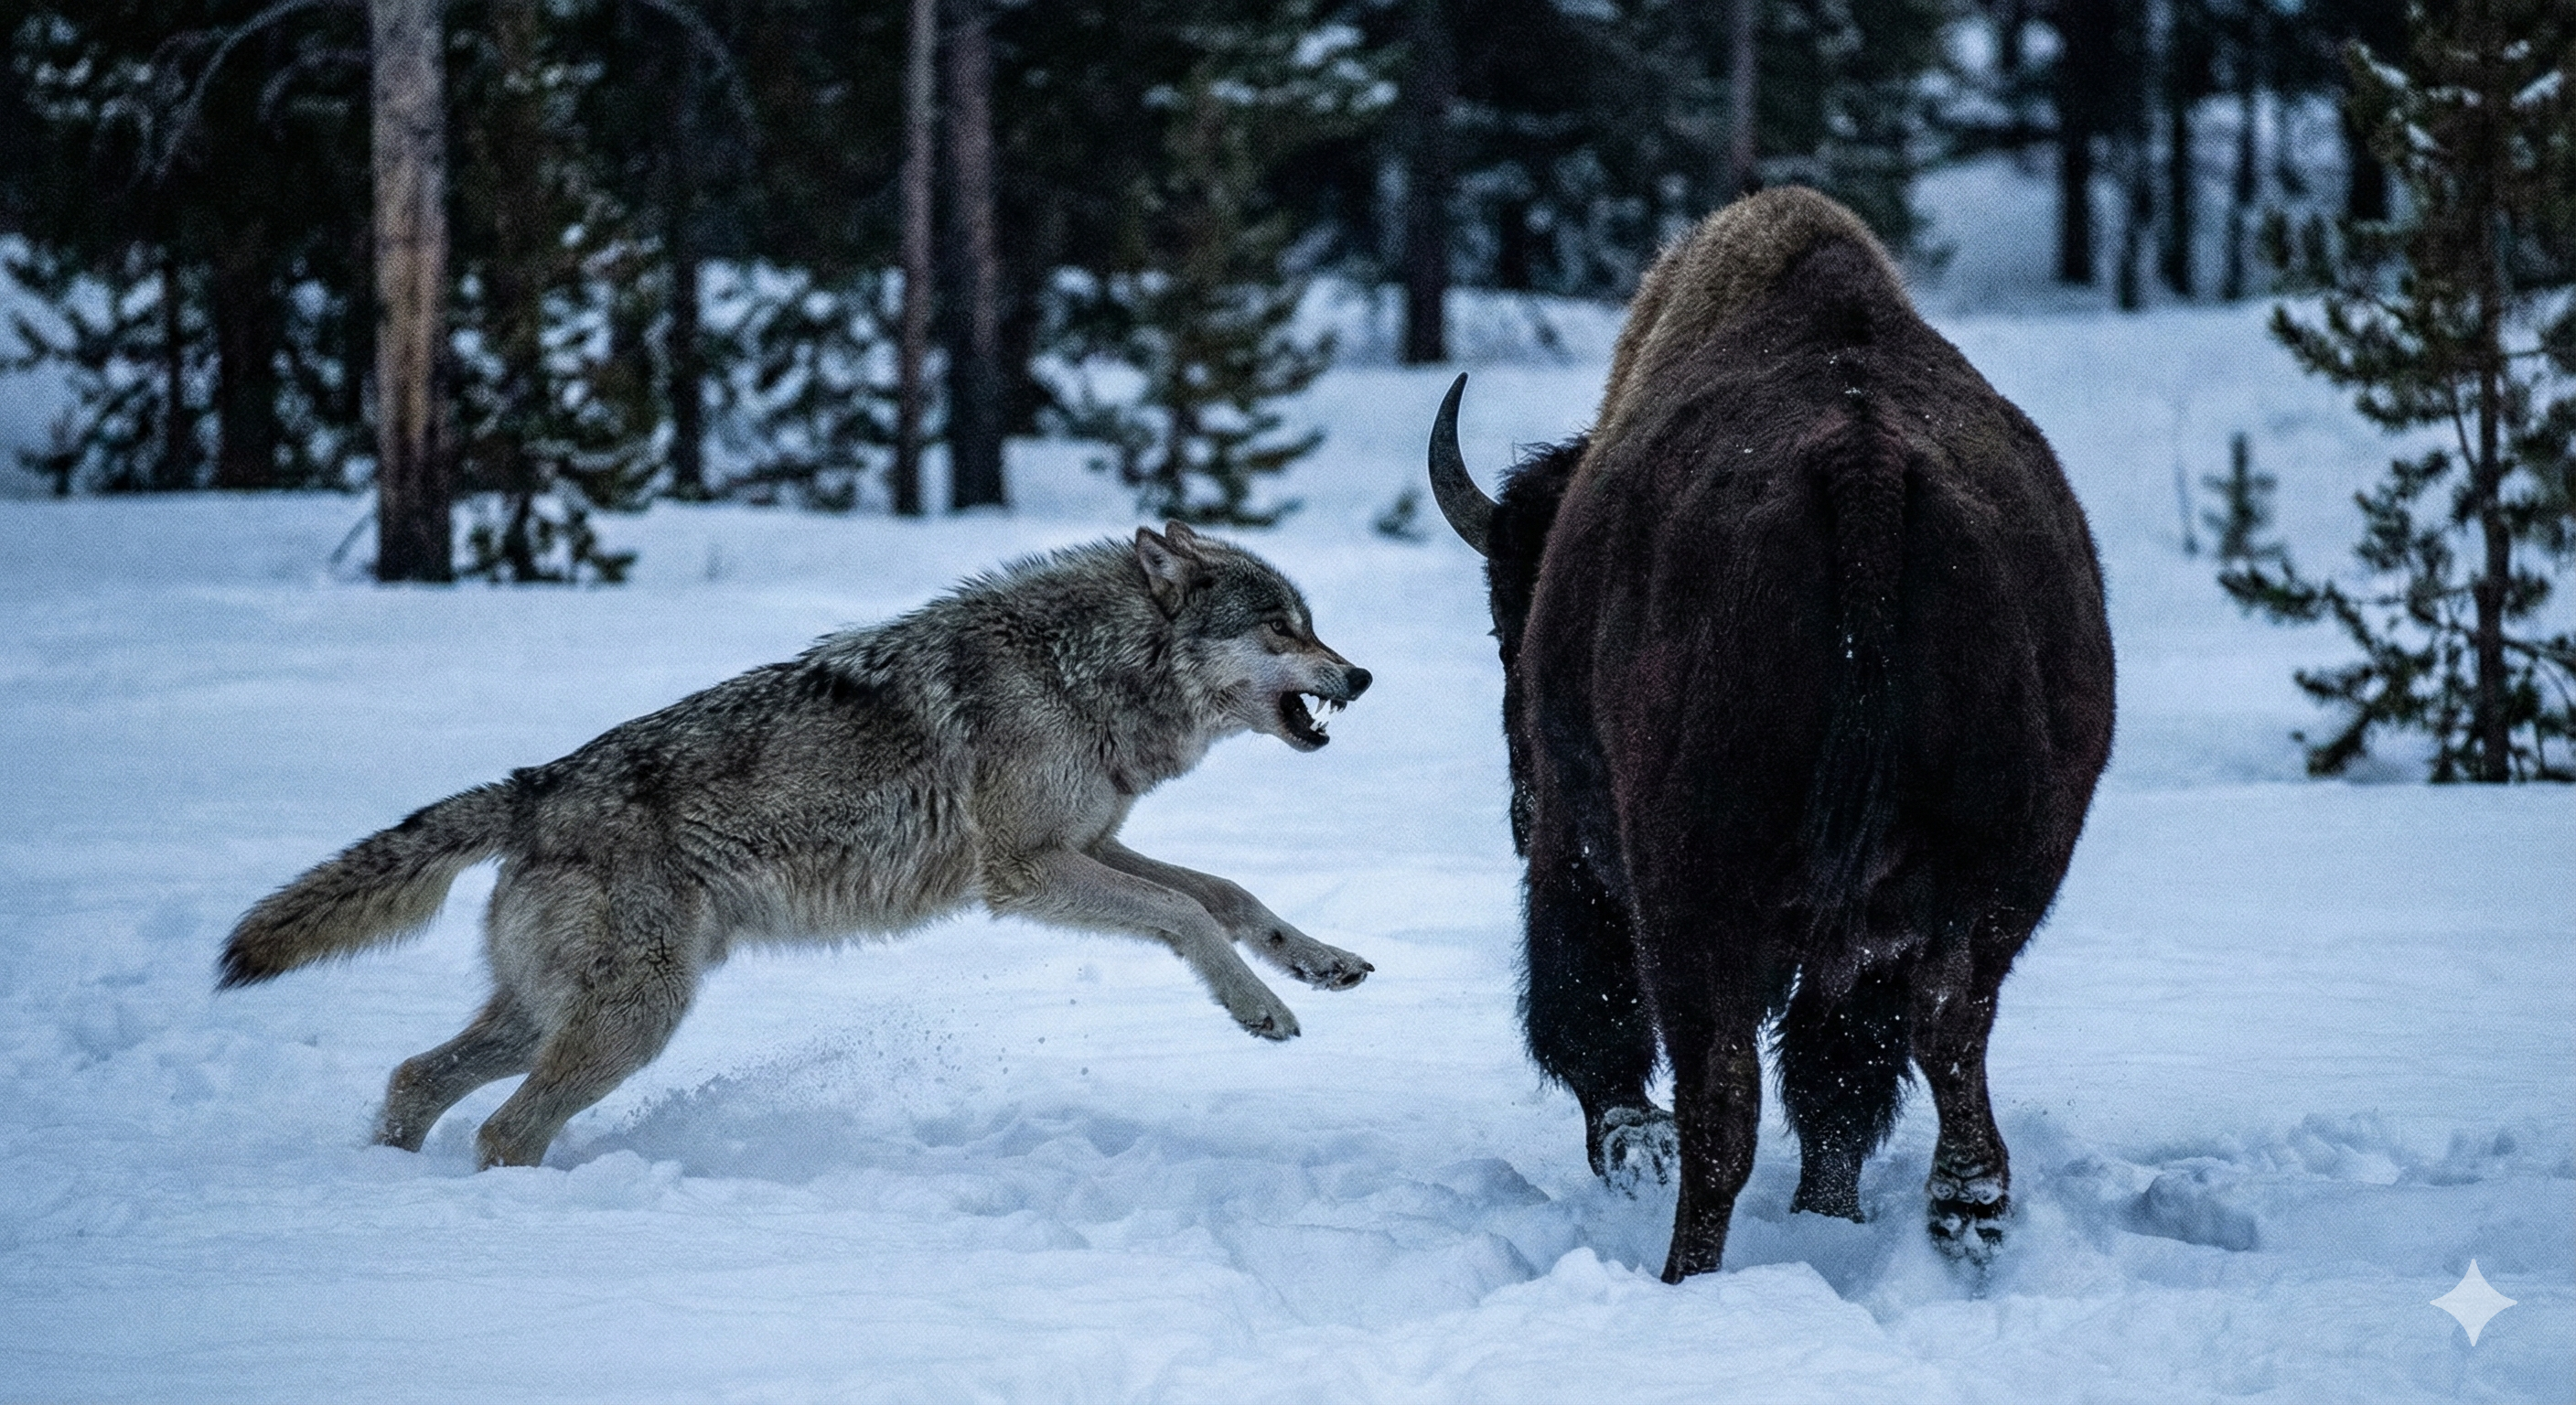
\includegraphics[width=350pt]{test_image_two.png}
    \caption{Example input image.}
    \label{fig:test_two}
\end{figure}

\begin{figure}[H]
    \centering
    \includegraphics[width=350pt]{two_q1.png}
    \caption{Example usage with other test image.}
    \label{fig:two_q1}
\end{figure}

\section{Conclusion}
In this project, the Moondream vision language model was successfully containerized using Docker. A Dockerfile was created to automate the installation of dependencies and the model itself, ensuring a consistent and reproducible environment. A Python script was developed to interface with the model, allowing users to perform Visual Question Answering tasks via a command-line interface. This implementation simplifies the deployment process and demonstrates the feasibility of running efficient VLMs on local hardware.

\begin{thebibliography}{9}

\bibitem{moondream}
Moondream.ai. \textit{Moondream: A tiny vision language model}. Available at: \url{https://moondream.ai/} (Accessed: \today).

\bibitem{huggingface}
Hugging Face. \textit{Hugging Face: The AI community building the future}. Available at: \url{https://huggingface.co/} (Accessed: \today).

\bibitem{docker}
Docker. \textit{Docker Documentation}. Available at: \url{https://docs.docker.com/} (Accessed: \today).

\bibitem{streamlit}
Streamlit. \textit{Streamlit: A faster way to build and share data apps}. Available at: \url{https://streamlit.io/} (Accessed: \today).

\end{thebibliography}

\end{document}
